\chapter{Experiments}

% TODO I cannot stress this enough times: make sure there is an explanation of heuristics notation used in pseudocode listing, SOMEWHERE

At this point of the thesis the reader should be already familiar with the notions we have introduced: the problem of finding the optimal ID set (with respect to a given \textit{weight}), that it is directly related to the NP-complete problem of finding the maximal weighted independent set, that this can be solved using the MIP approach, and that there are several possibilities how to optimize the work of the solver by employing various heuristics.

We have implemented these ideas and incorporated them in the jInfer framework (see Appendix \ref{appedix-jInfer}). But before we describe the experiments themselves, we should try to formulate our aim.\\

First of all, we describe how the whole system and its components behave. We want to see the changes introduced by modifying several parameters, while keeping the others fixed. They probably will not be orthogonal, we might at least isolate some of the parameters that are less important to the overall behavior.

Second, we evaluate the system performance in terms of the speed of finding good heuristic results. We find tweaks to make the whole process as fast as reasonably possible.

And in the end, we formulate general recommendations regarding the problem of finding ID sets.

\section{Experimental Data}
\label{section-experiments-data}

To conduct out experiments, we are using XML documents of three categories:

\begin{itemize}
	\item Realistic
	\item Realistic with artificial (converted) attributes
	\item Artificial
\end{itemize}

In case of realistic data we want to see the performance in cases taken from the real world. The problem with realistic data is that sometimes, interesting values (that might or might not contain IDs) are stored as simple text nodes instead of attributes. We will try to convert some of these values to attributes (e.g. using a smart XSL transformation), let our heuristics find the ID sets, and then translate them back to XML keys (see Section \ref{section-realistic-converted} for details).
And finally, we create completely artificial data to create inputs that will put our heuristics in stress. This is because the realistic data often prove to be too simple to solve - the list of candidate AMs is usually too short to be hard to be solved to optimality.

\begin{define}[Data set]
	\label{define-data-set}
	One or more XML files sharing the same schema (even if only an implicit schema) shall be referred to as a \textit{data set}. In the scope of this work this will always mean a \textit{single} XML file. However, this definition of a data \textit{set} covers also the extension to more XML files as described in \cite{fidax}.
\end{define}

To understand our test data sets we discuss their origin and \textit{graph representation}. As mentioned earlier, % TODO link
the problem of finding the optimal ID set is in fact the problem of finding the maximum weighted independent set in a graph. Therefore it is interesting to actually see the graphs of these data sets and understand some related metrics.

The former will be achieved with the help of the GraphViz tool (\cite{graphviz}), where we will draw the graphs so that all the vertices represent the \textit{candidate AMs}, and the edges represent pairs of AMs that have nonempty intersection of their images (and thus cannot be in the same ID set together). Thus solving the maximal weighted IS on these graphs will be equivalent to solving our problem of optimal ID set.

The latter will come in form of tables containing information regarding the data sets, such their size, known optimum for $\alpha = \beta = 1$ (found by running the \heu{Glpk} heuristic without a time limit) and the numbers of vertices and edges in aforementioned graphs.

\subsection{Realistic data}
\label{section-realistic-data}

From 3 different sources we collected 6 different data sets, called \dataset{OVA1} - \dataset{OVA3}, \dataset{XMA-c}, \dataset{XMA-p} and \dataset{XMD}. Their summary is Table \ref{table-experiments-data-realistic}, their graph representations can be seen in Figure \ref{image-experiments-data-realistic}. Because the legal status of disclosing these data sets is unclear, we will refrain from identifying them beyond these artificial identifiers. Neither will they be included on the DVD distributed with this thesis.

\begin{table}
  \caption{List of realistic test data files}
  \bigskip
  \label{table-experiments-data-realistic}
  \centering
  \begin{tabular}{l | r | c | c | l}
  	Name  & Size [kb] & $|V|$ & $|E|$ & Optimum \\
  	\hline
  	\dataset{OVA1}  & 4.5      & 29 & 43 & 0.45588235294117635 \\
  	\dataset{OVA2}  & 11.9     & 23 & 36 & 0.1634615384615385  \\
  	\dataset{OVA3}  & 237.6    & 31 & 47 & 0.25537156151635415 \\
  	\dataset{XMA-c} & 1 807.7  & 1  & 0  & 0.7546666666666667  \\
  	\dataset{XMA-p} & 13 748.3 & 1  & 0  & 0.2019306150568969  \\
  	\dataset{XMD}   & 1 743.0  & 17 & 15 & 0.09786094165493507 \\
  \end{tabular}
\end{table}

\begin{figure}
  \caption{Realistic data}
  \label{image-experiments-data-realistic}
  \centering
    \subfigure[\dataset{OVA1}]{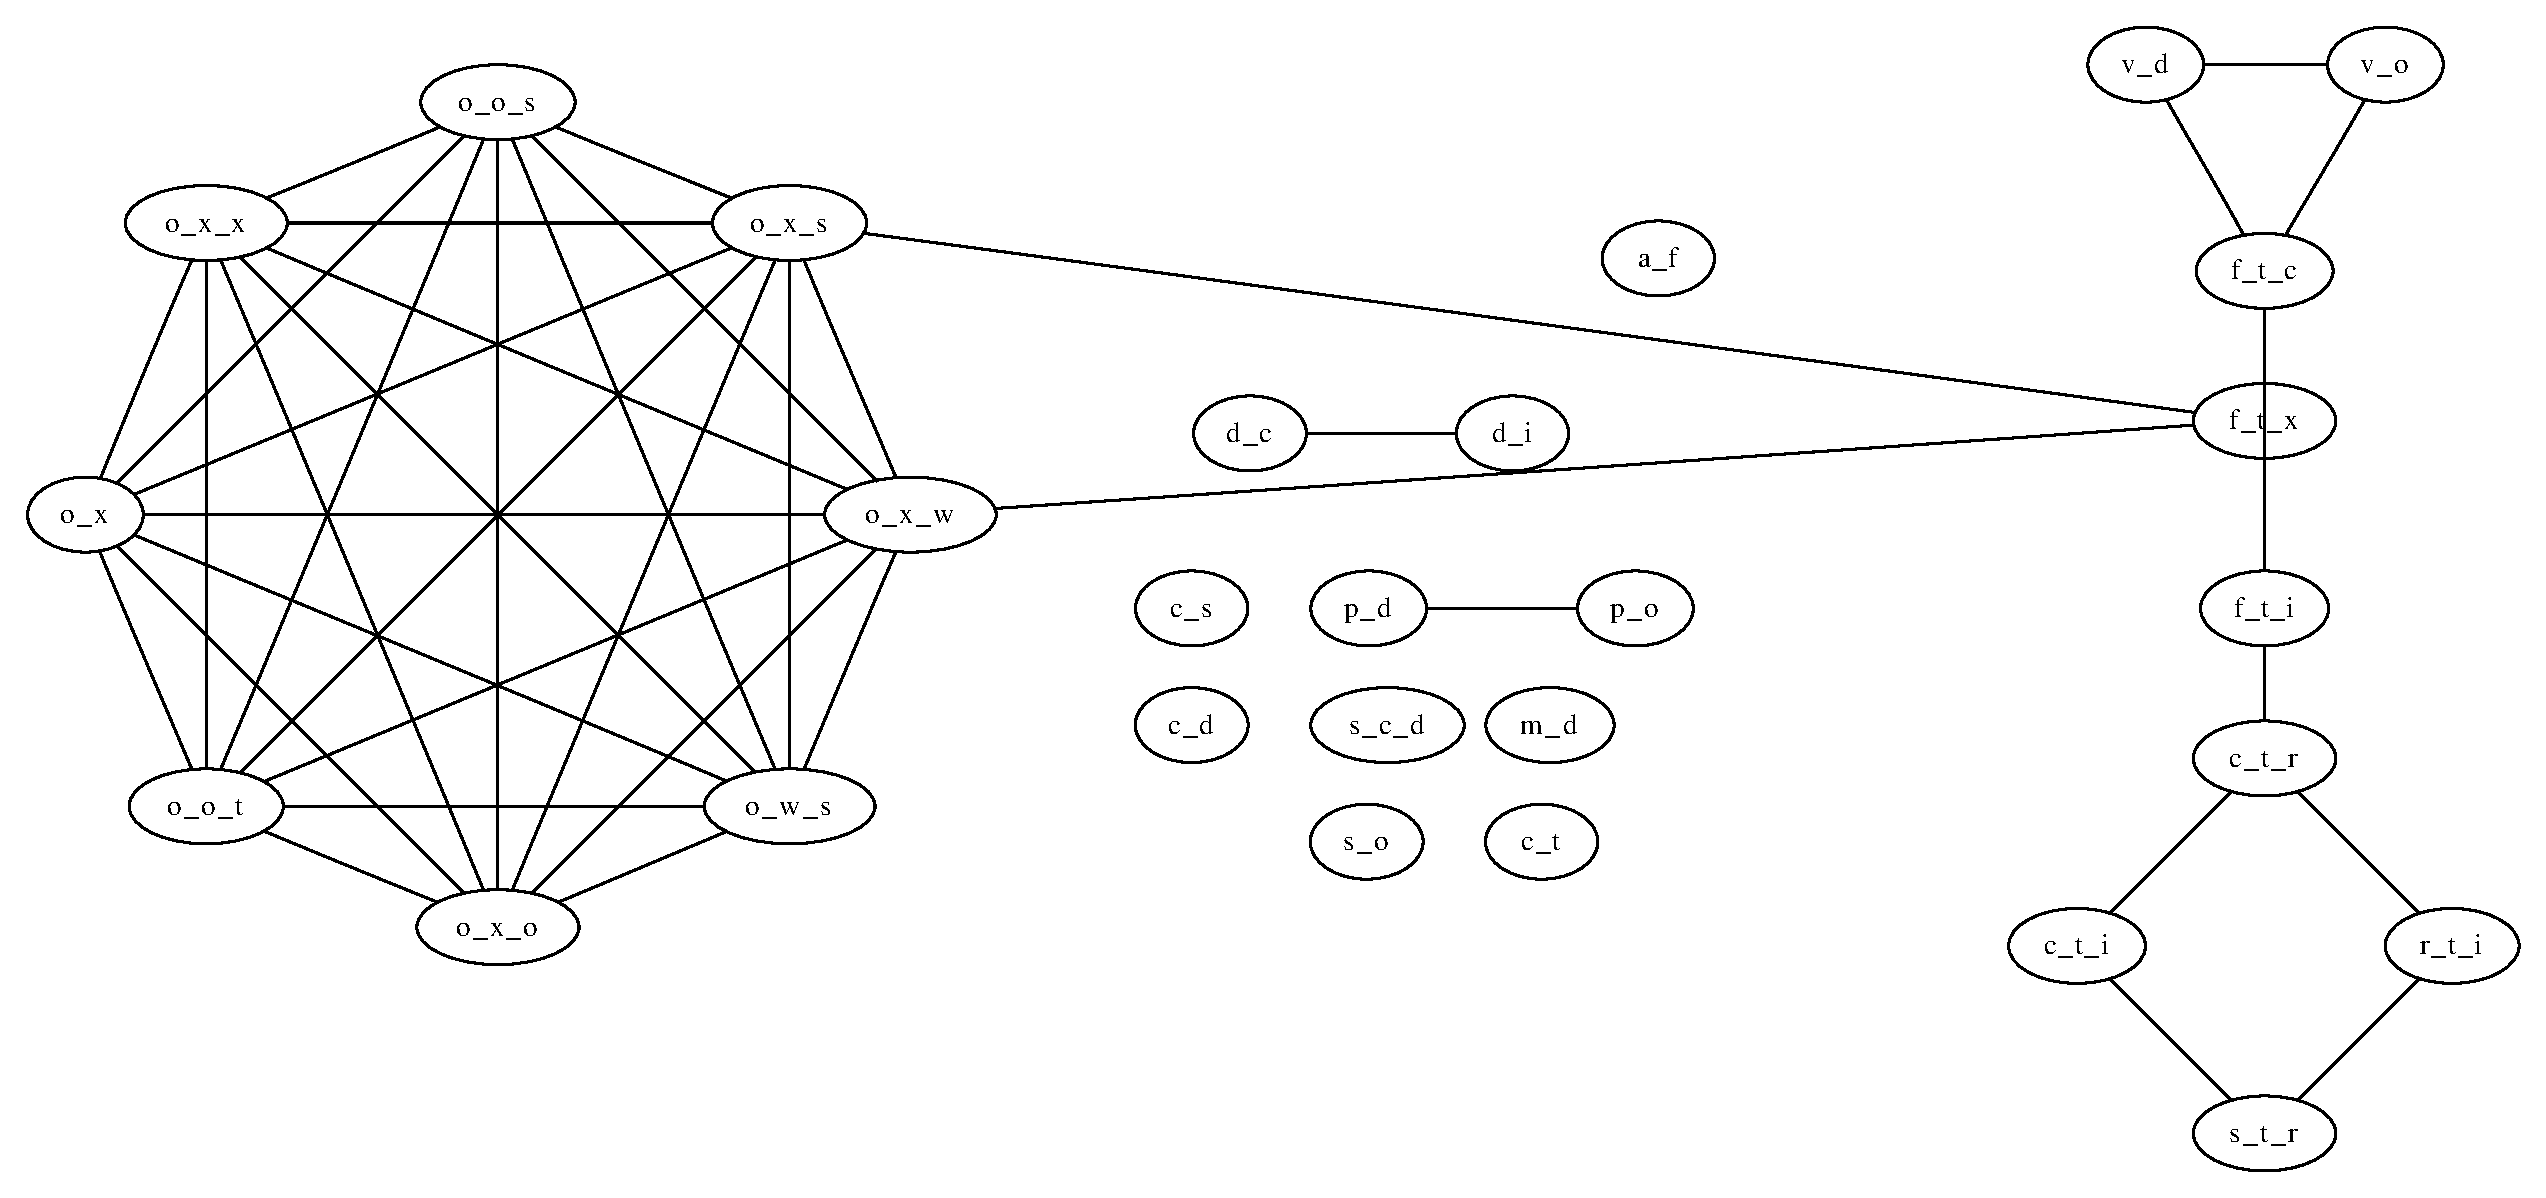
\includegraphics[width=0.45\textwidth]{images/experiments/data/realistic/OVA1}}
    \subfigure[\dataset{OVA2}]{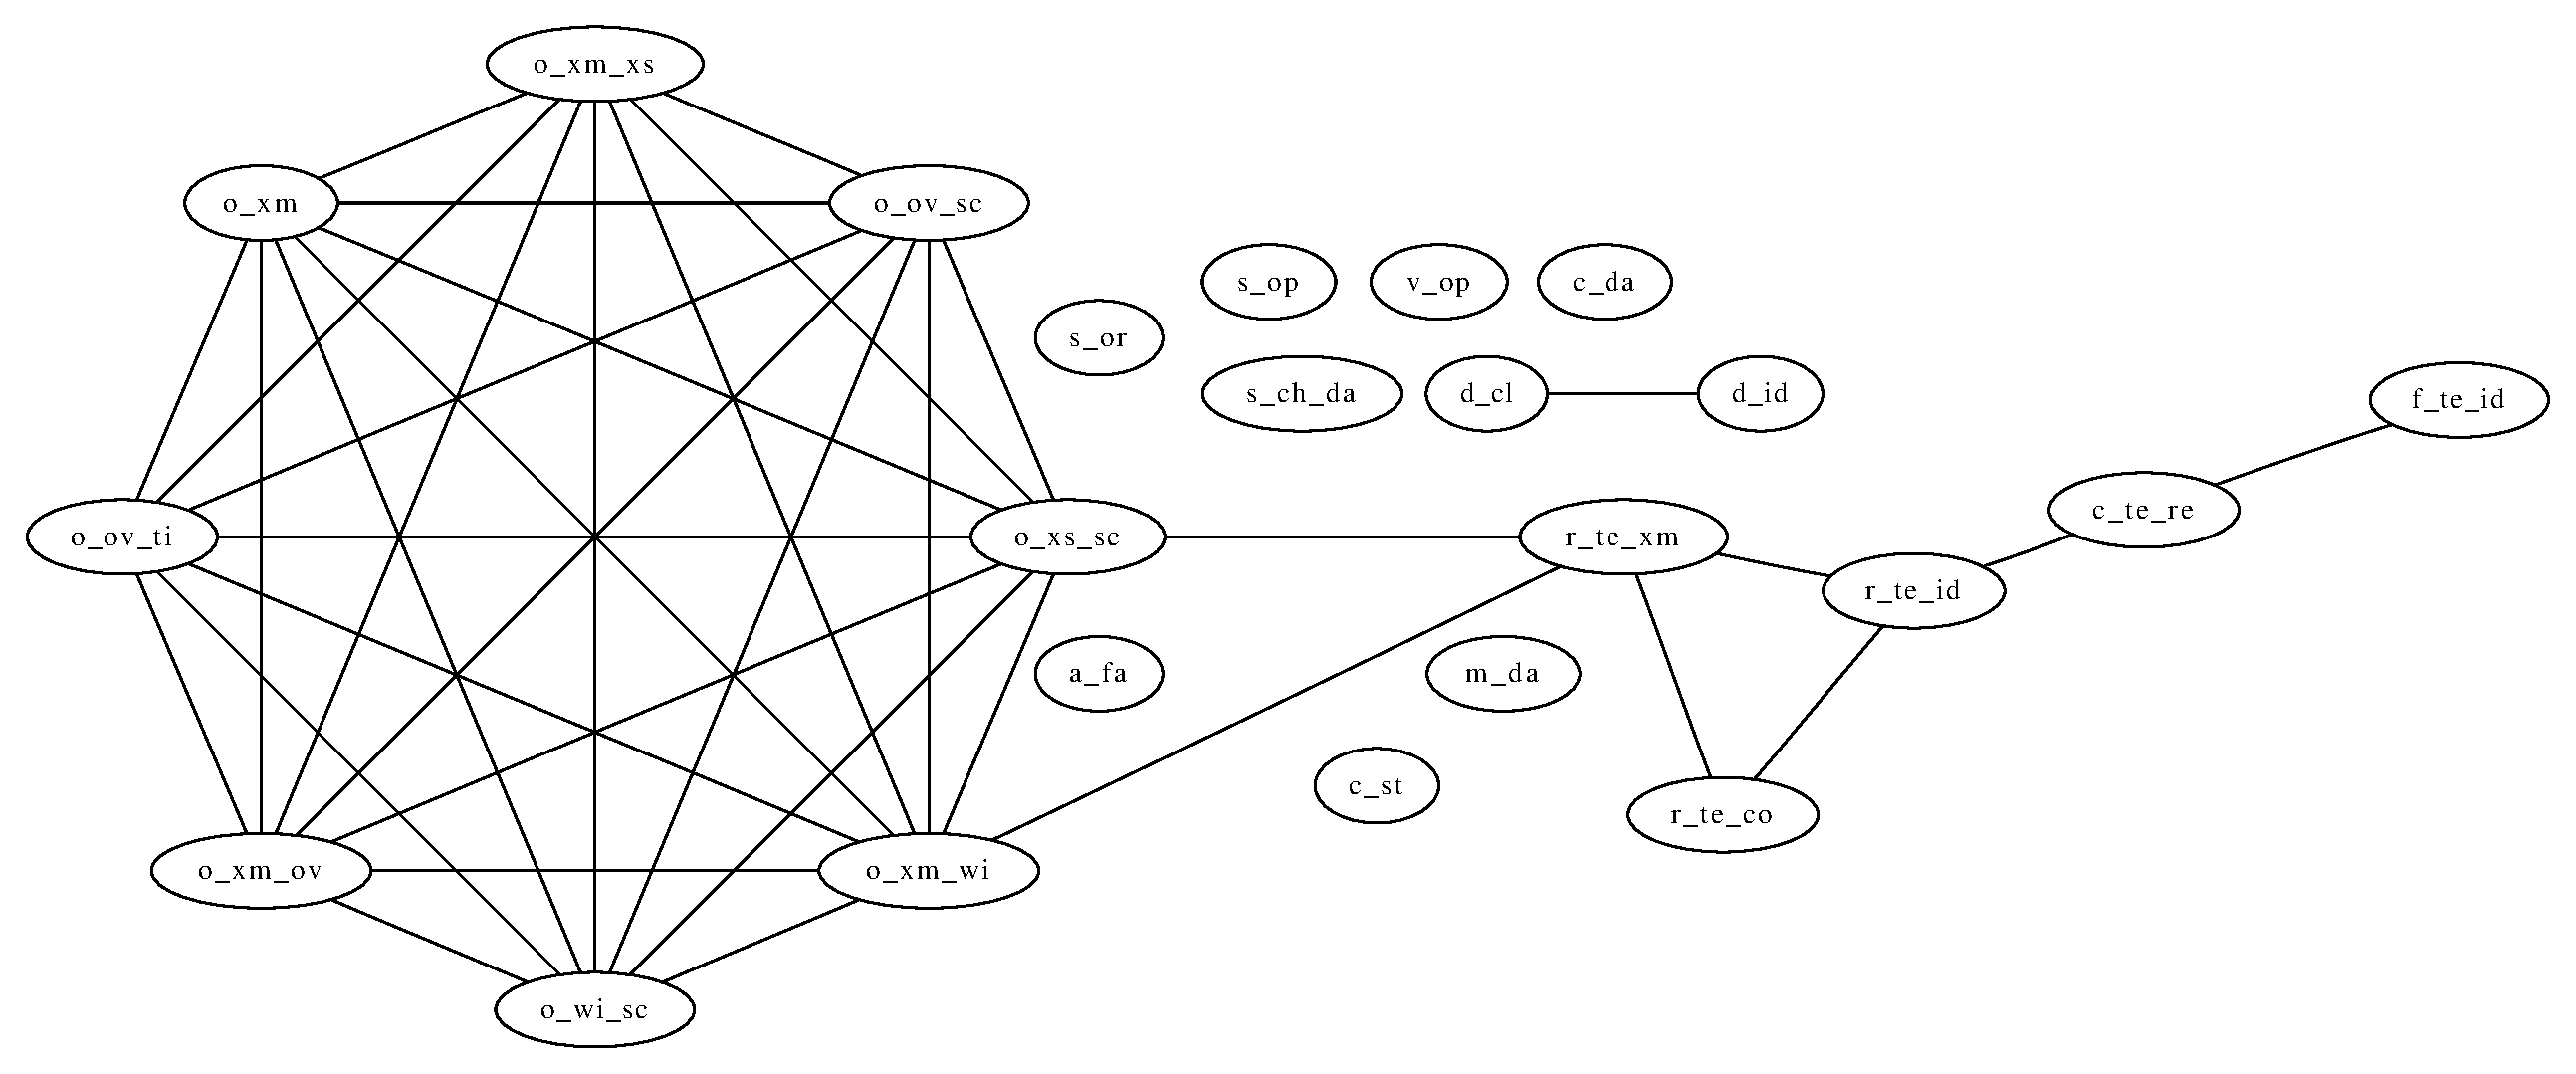
\includegraphics[width=0.45\textwidth]{images/experiments/data/realistic/OVA2}}
    \subfigure[\dataset{OVA3}]{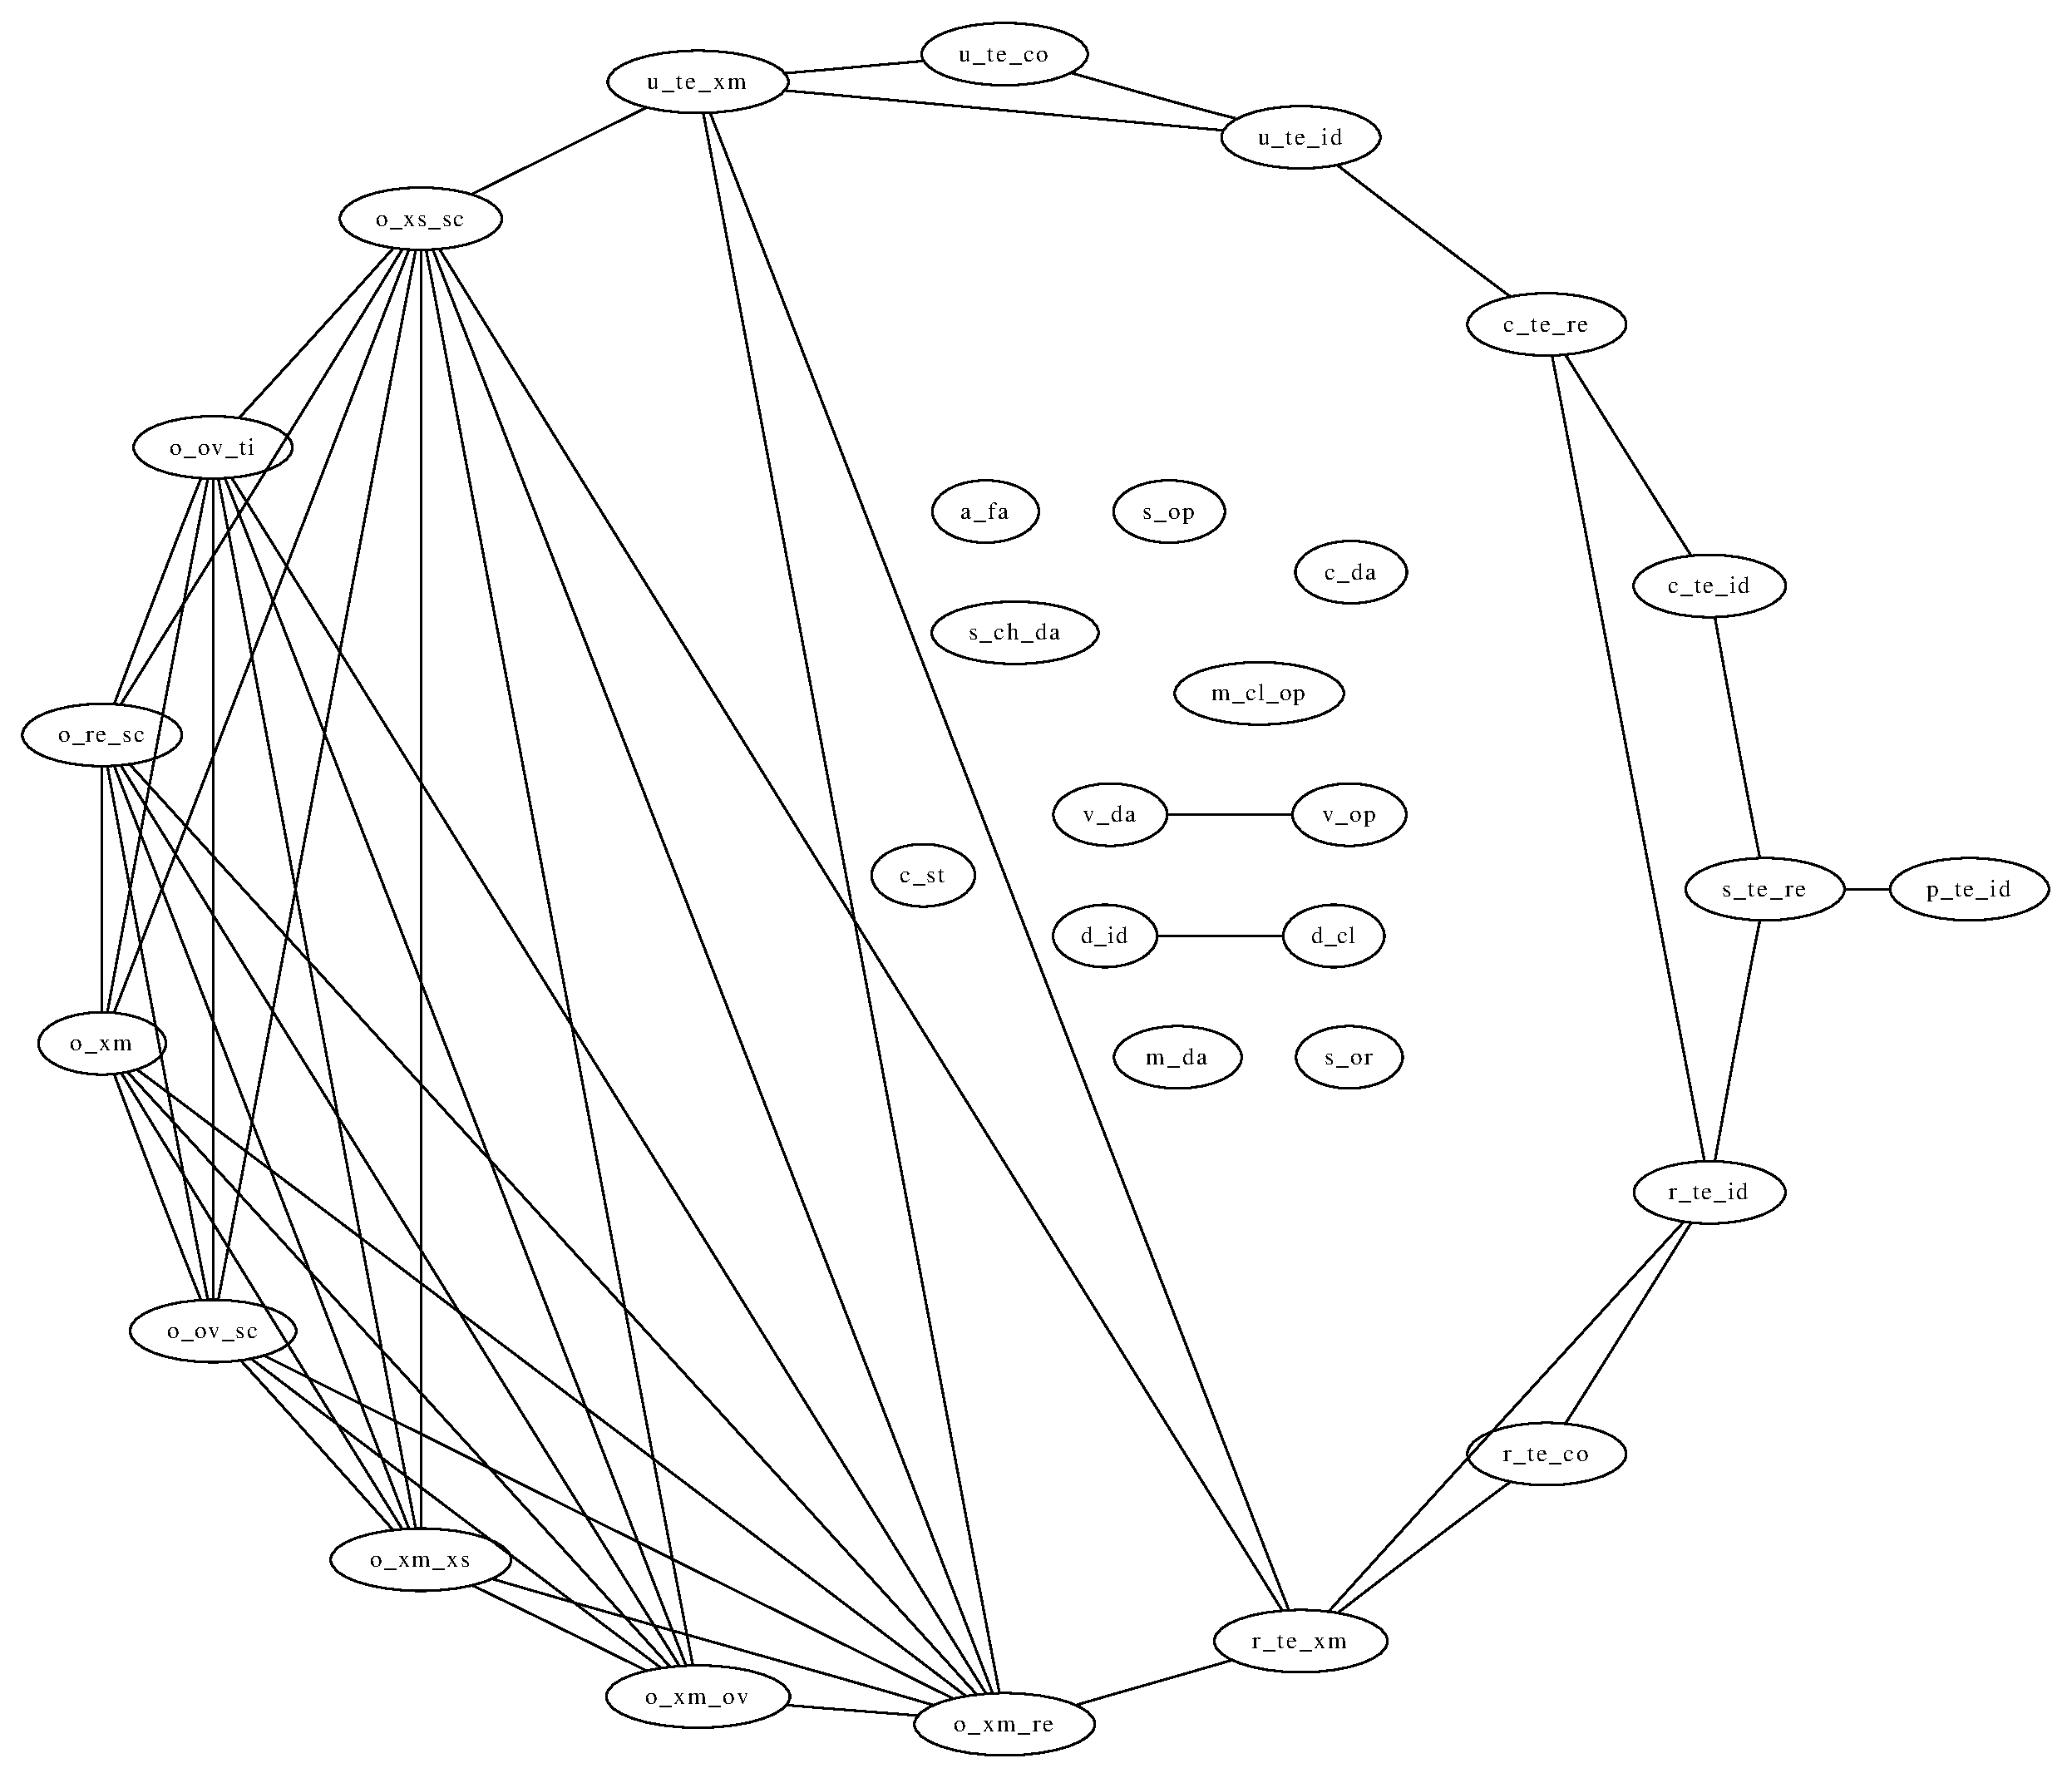
\includegraphics[width=0.45\textwidth]{images/experiments/data/realistic/OVA3}}
    \subfigure[\dataset{XMA-c}]{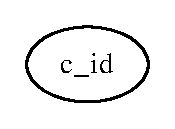
\includegraphics[width=0.08\textwidth]{images/experiments/data/realistic/XMA-c}}
    \subfigure[\dataset{XMA-p}]{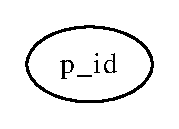
\includegraphics[width=0.08\textwidth]{images/experiments/data/realistic/XMA-p}}
    \subfigure[\dataset{XMD}]{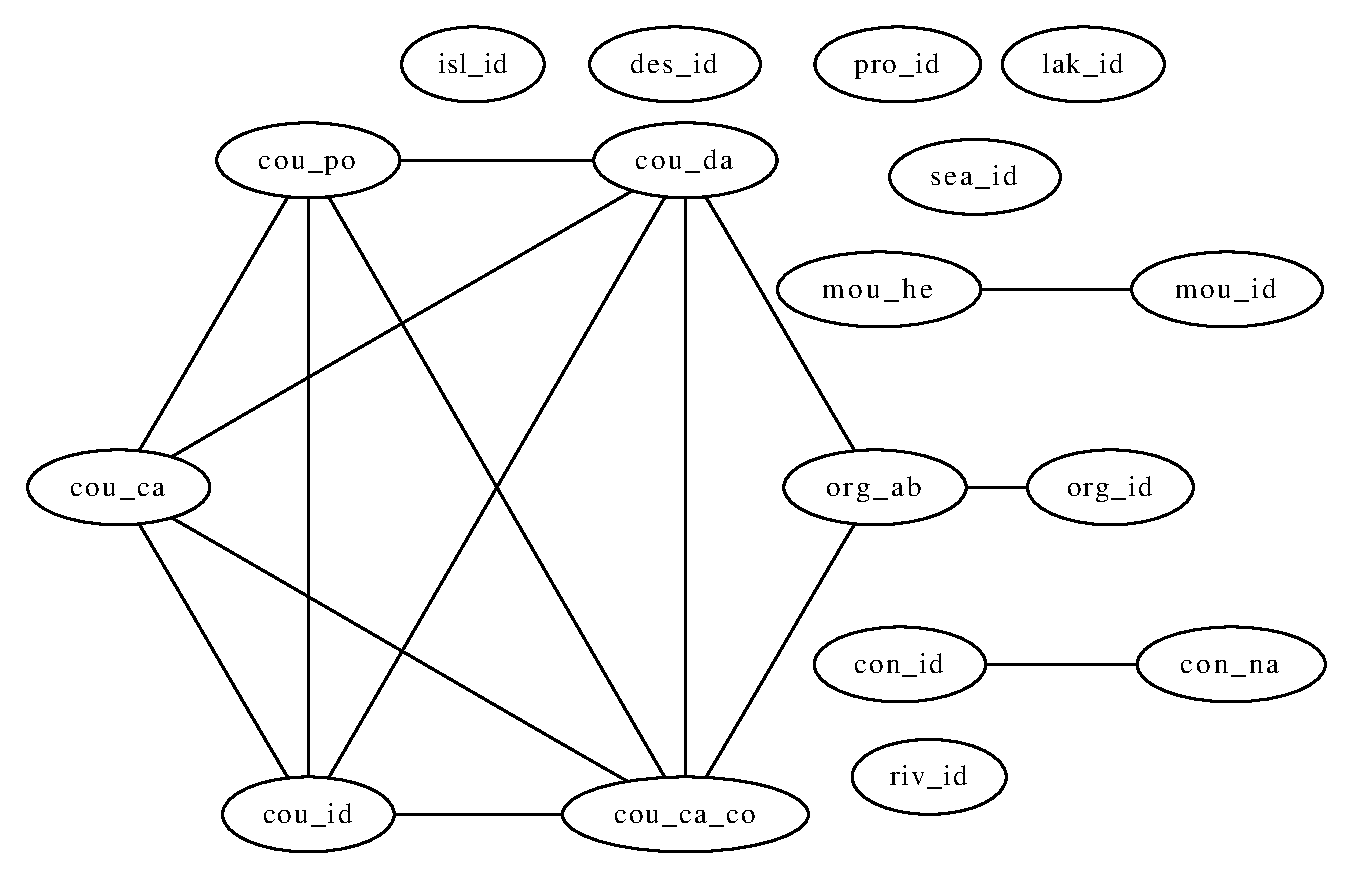
\includegraphics[width=0.45\textwidth]{images/experiments/data/realistic/XMD}}
\end{figure}

To interpret the data: \dataset{OVA*} sets have quite interesting and challenging graphs, but they are relatively small. We can consider them to be the ``typical" representants.

On the other hand, the \dataset{XMA-*} sets are relatively huge, but trivial: their only candidate AM will just get picked and the heuristic will end. Therefore we will see the performance of the other components of the whole system, such as loading the data sets into memory representations.

Finally, the \dataset{XMD} set is relatively big and, at the same time, has non-trivial graph representation. In this case we should see a performance more balanced between processing and finding the ID set.

\subsection{Realistic data with artificial attributes}
\label{section-realistic-converted}

We used 2 data sets to convert, \dataset{MSH} and \dataset{NTH}. Unfortunately, the same problem with disclosure as in the previous case applies here. None of these sets had any attributes before the conversion. Their summary is Table \ref{table-experiments-data-converted}, their graphs are in Figure \ref{image-experiments-data-converted}.

To address the conversion: in case of \dataset{MSH} we found 2 elements with values resembling a key of the records contained in the file, and converted them to be attributes of these records using a simple XSL transformation. In the case of \dataset{NTH} we converted all the values in sub-elements of the record elements to be the attributes of the records.

This approach is useful, because as stated in TODO link, ID attributes are a special case of XML keys. We can use this approach to find XML keys: convert some ``suspicious" data into attributes, find the optimal ID set and then create XML key based on this ID set.

\begin{table}
  \caption{List of realistic test data files with converted attributes}
  \bigskip
  \label{table-experiments-data-converted}
  \centering
  \begin{tabular}{l | r | c | c | l}
  	Name  & Size [kb] & $|V|$ & $|E|$ & Optimum \\
  	\hline
  	\dataset{MSH}  & 3 100.5 & 1 & 0 & 0.5416472778036296 \\
  	\dataset{NTH}  & 2 523.5 & 5 & 7 & 0.057918595422124436 \\
  \end{tabular}
\end{table}

\begin{figure}
  \caption{Realistic data with converted attributes}
  \label{image-experiments-data-converted}
  \centering
    \subfigure[\dataset{MSH}]{
\includegraphics[width=0.08\textwidth]{images/experiments/data/converted/MSH}}
    \subfigure[\dataset{NTH}]{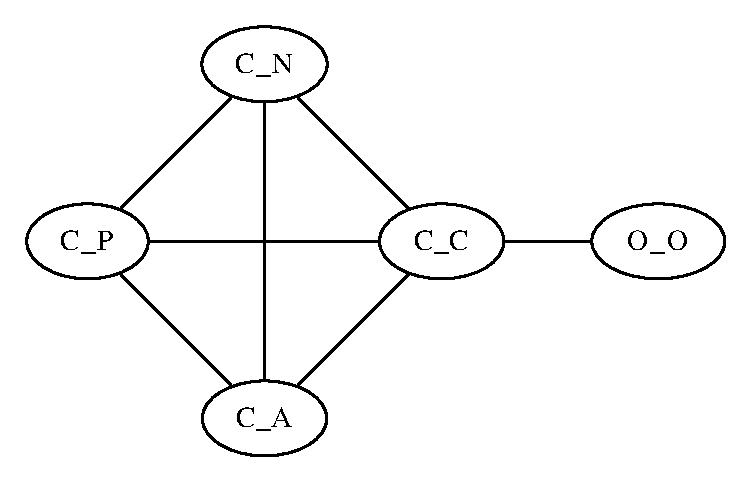
\includegraphics[width=0.45\textwidth]{images/experiments/data/converted/NTH}}
\end{figure}

In case of \dataset{MSH} we created 2 attributes, of which only one constituted a candidate AM. This is then the case similar to \dataset{XMA-*} sets: quite large data, yet only one trivial ID attribute to be found.

In case of \dataset{NTH} we introduced 8 attributes. Out of them 5 proved to be candidate AMs, with 7 edges constraining them. This means we have a relatively large set with considerably simple work to be done by the heuristics.

\subsection{Artificial data}

As soon as we started experimenting with the data coming from the real world, it was obvious that they are not complex enough. After we built the model, we got the most complex graphs of 31 vertices and 47 edges (see Table \ref{table-experiments-data-realistic}). Our solution is to approach the problem from the other side: in the end, we will be solving the equivalent of IS problem on a graph created from XML data. We will create the XML data to contain a more complex graph with a specific number of vertices and edges.

To demonstrate this, consider the following excerpt from an XML file:

\begin{scriptsize}
\begin{verbatim}
<graph>
  <vertex0 attr="-2968876296119015800"/>
  <vertex1 attr="1729745997570096518"/>
  <vertex2 attr="-9020549659620928934"/>
  ...
  <vertex99 attr="-7545982394508643394"/>

  <vertex82 attr="0"/><vertex21 attr="0"/>
  <vertex64 attr="1"/><vertex21 attr="1"/>
  <vertex44 attr="2"/><vertex2 attr="2"/>
  ...
  <vertex96 attr="99"/><vertex40 attr="99"/>
</graph>
\end{verbatim}
\end{scriptsize}

Our aim is to create a graph with approximately $v$ vertices and $e$ edges. First, we introduce $v$ elements with names \texttt{vertex0} - \texttt{vertex\{V-1\}}. To constitute an AM, they need an attribute \texttt{attr}, but with large enough random values, so that they do not conflict with others. Second, for each of the $e$ edges we choose two \texttt{vertex*} elements at random, and give them the same value of their \texttt{attr}. This will ensure they cannot share the same ID set, thus effectively creating the edge in the graph representation.

The respective pseudocode for this is provided in Algorithm \ref{listing-random-data}.

\begin{algorithm}
\caption{Random XML data creation}
\label{listing-random-data}
\begin{algorithmic}
\REQUIRE $v$ requested number of vertices
\REQUIRE $e$ requested number of edges
\ENSURE XML file content
\PRINT \texttt{<graph>}
\FOR{$i = 1 \to |V|$}
	\STATE $R \gets RANDOM$
	\PRINT \texttt{<vertex\textit{i} attr="\textit{R}">}
\ENDFOR
\FOR{$i = 1 \to |E|$}
	\STATE $v1 \gets RANDOM(|V|)$
	\STATE $v2 \gets RANDOM(|V|)$
	\PRINT \texttt{<vertex\textit{v1} attr="\textit{i}"> <vertex\textit{v2} attr="\textit{i}">}
\ENDFOR
\PRINT \texttt{</graph>}
\RETURN
\end{algorithmic}
\end{algorithm}

With this process it is possible to create as much data as needed, with any combination of $v$ and $e$ requested.

There is one characteristic that can describe random graphs like this, and that is the \textit{density}. This can be defined in various ways, we will use two different interpretations. The first is $\frac{|E|}{|V|}$, that is, how many edges are there for one vertex (multiplied by 2 we would get the average degree of the vertices).

The second, perhaps more interesting is $\frac{|E|}{E_{max}}$, where $E_{max} = \frac{|V|.(|V|-1)}{2}$. This is the density as the ratio of edges that are to all edges that could be in a complete graph with $|V|$ vertices.

We have created 3 sets to be used in experiments along with the realistic and converted sets, called \dataset{100-100}, \dataset{100-200} and \dataset{100-1000}. Note that the name is always in the form $v-e$.\\

All of the experimental data sets mentioned so far, realistic, converted and artificial alike will be referred to as \textit{official test data (sets)}.\\

Also, we will need data of comparably similar characteristics but varying size to study the effects of size on the run times of experiments. For this reason we created 11 more sets, from \dataset{0-0} as the trivial one to \dataset{100-500} as the largest one. These will be referred to as \textit{sized test data (sets)}. We wanted to keep the same density among these sets, so we picked the $\frac{|E|}{E_{max}}$ density interpretation for this.

A summary is provided in Table \ref{table-experiments-data-artificial} and Table \ref{table-experiments-data-artificial-size}; these tables contain 2 new columns: values of density in both interpretations we introduced. Some of the graph representations can be seen in Figure \ref{image-experiments-data-artificial}.

While studying the tables it becomes obvious that the actual numbers $|V|$ and $|E|$ do not match to the $v$ and $e$ in the names of the sets. This is because of the way the random generation algorithm works: it might pick the same edge twice, which will automatically render it unsuitable for the ID set. Because of the so-called Birthday paradox (see e.g. \cite{birthday}), this will happen more with higher $e$.

\begin{table}
  \caption{List of artificial test data files}
  \bigskip
  \label{table-experiments-data-artificial}
  \centering
  \begin{tabular}{l | r | c | c | c | c | l}
  	Name  & Size [kb] & $|V|$ & $|E|$ & $\frac{|E|}{|V|}$ & $\frac{|E|}{E_{max}}$ & Optimum \\
  	\hline
  	\dataset{100-100}  & 8.4  & 99 & 95  & 0.95 & 0.02 & 0.836666666666667 \\
  	\dataset{100-200}  & 13.0 & 96 & 174 & 1.81 & 0.04 & 0.726000000000000 \\
    \dataset{100-1000} & 49.5 & 93 & 754 & 8.11 & 0.16 & 0.380952380952381 \\
  \end{tabular}
\end{table}

\begin{table}
  \caption{List of ``sized" artificial test data files}
  \bigskip
  \label{table-experiments-data-artificial-size}
  \centering
  \begin{tabular}{l | r | c | c | c | c | l}
	  Name  & Size [kb] & $|V|$ & $|E|$ & $\frac{|E|}{|V|}$ & $\frac{|E|}{E_{max}}$ & Optimum \\
  	\hline
  	\dataset{0-0}     & 0.2  & 0  & 0   & -    & -    & 0.0                \\
  	\dataset{10-5}    & 0.6  & 10 & 5   & 0.50 & 0.11 & 0.8500000000000002 \\
    \dataset{20-20}   & 1.7  & 18 & 13  & 0.72 & 0.08 & 0.7166666666666669 \\
    \dataset{30-45}   & 3.1  & 29 & 43  & 1.48 & 0.11 & 0.7083333333333334 \\
  	\dataset{40-80}   & 5.1  & 39 & 72  & 1.85 & 0.10 & 0.6950000000000002 \\
  	\dataset{50-125}  & 7.5  & 48 & 111 & 2.31 & 0.10 & 0.6566666666666666 \\
  	\dataset{60-180}  & 10.4 & 58 & 157 & 2.71 & 0.09 & 0.6214285714285716 \\
  	\dataset{70-245}  & 13.8 & 67 & 205 & 3.06 & 0.09 & 0.5982142857142856 \\
  	\dataset{80-320}  & 17.6 & 76 & 261 & 3.43 & 0.09 & 0.5791666666666667 \\
  	\dataset{90-405}  & 21.9 & 86 & 352 & 4.09 & 0.10 & 0.528888888888889  \\
  	\dataset{100-500} & 26.7 & 91 & 388 & 4.26 & 0.09 & 0.4981818181818182 \\
  \end{tabular}
\end{table}

\begin{figure}
  \caption{Artificial data}
  \label{image-experiments-data-artificial}
  \centering
  	\subfigure[\dataset{48-80}]{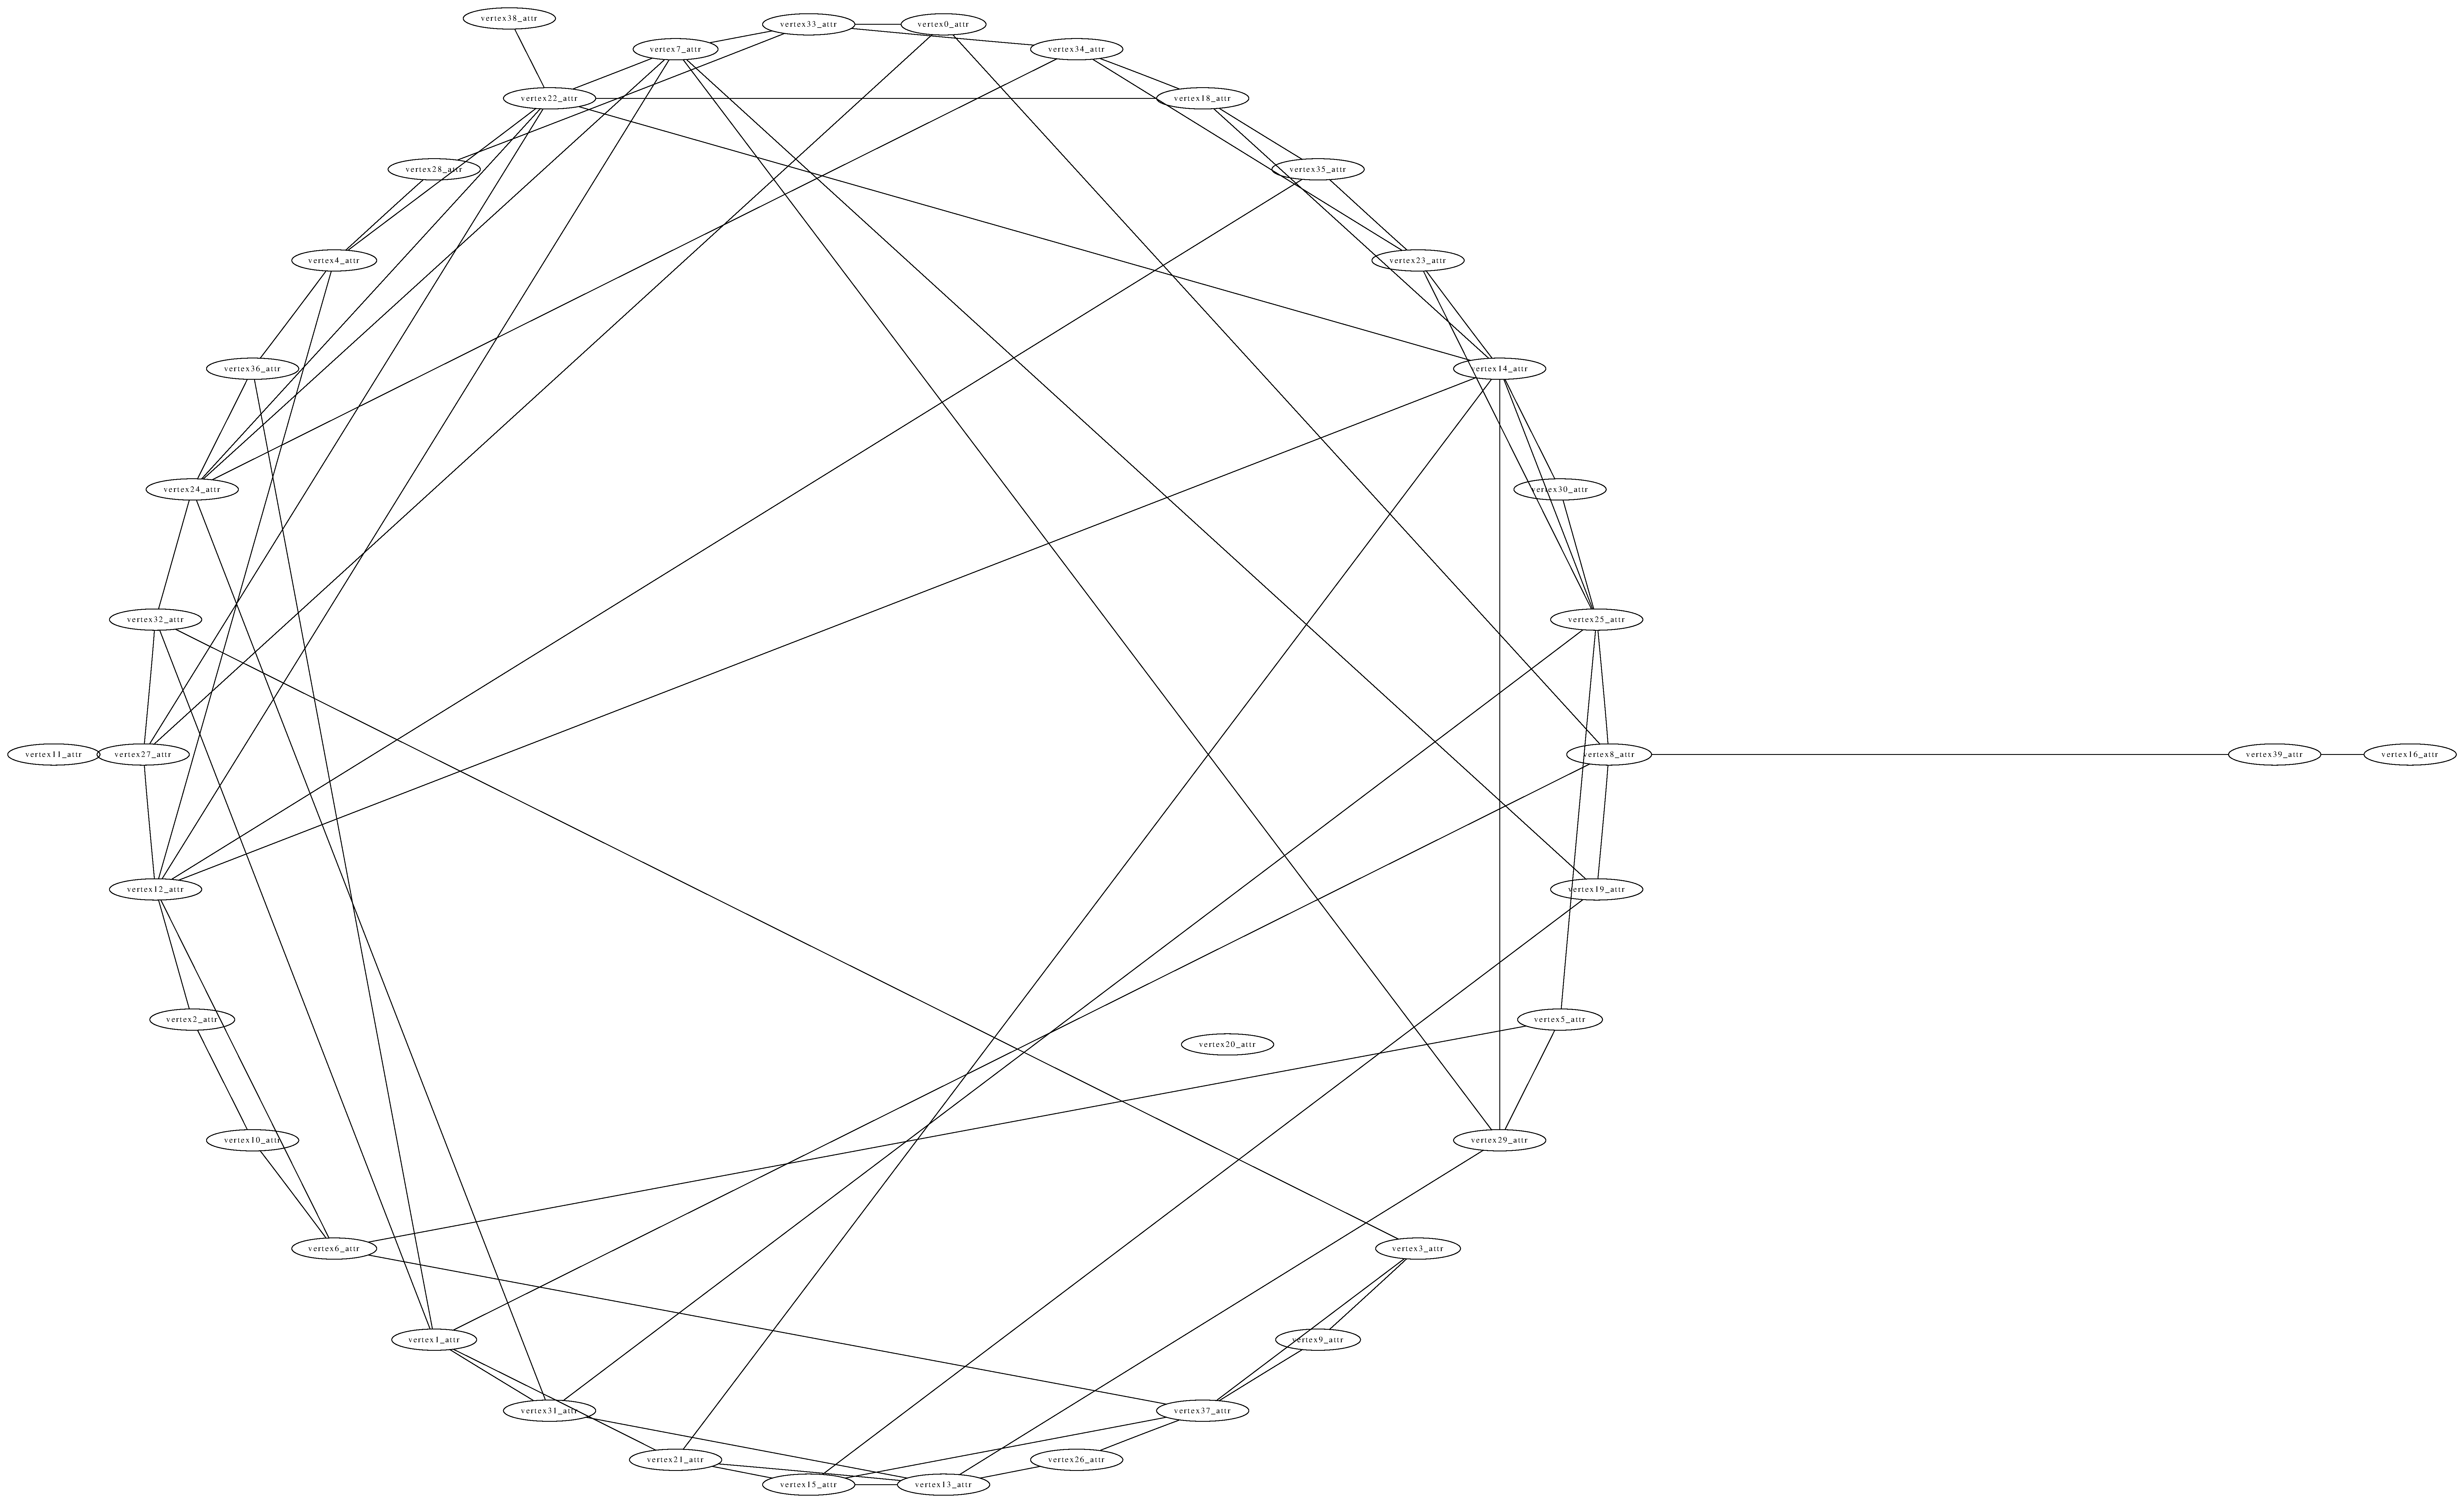
\includegraphics[width=\textwidth]{images/experiments/data/artificial/size/40-80}}
	\subfigure[\dataset{70-245}]{
\includegraphics[width=\textwidth]{images/experiments/data/artificial/size/70-245-fixed}}
\end{figure}

To interpret Tables \ref{table-experiments-data-artificial} and \ref{table-experiments-data-artificial-size}: we get 3 sets of different sizes and densities in the first one. The $|V|$ and $|E|$ numbers are orders of magnitude higher than in any realistic (or converted) data set we are using.

In the second table we aimed for the $\frac{|E|}{E_{max}}$ density of $0.1 = 10\%$, and we can see that this was indeed achieved. There is an interesting observation to be made here: the optimum is steadily decreasing with the increasing overall graph size. This intuitively suggests that the maximum quality theoretically achievable is related to the $\frac{|E|}{|V|}$ density, not to the one we fixed. Exploration of this phenomenon is beyond the scope of this thesis.

Note that the artificial data we used in experiments can be found on the DVD enclosed with this work.

\section{Experimental Setup}

As was mentioned before, we will use an extension to the jInfer framework called \jmodule{IDSetSearch}. Please see Appendices \ref{appendix-jInfer} and \ref{appendix-iss} for more detailed information on these two pieces of software.\\

We now have to introduce a few notions before moving forward to the description of our experiments.\\

\textit{Experiment parameters} are the following ones.
\begin{itemize}
	\item All the parameters in all the heuristics.
	\item The specific way in which the heuristics are chained.
	\item Parameters $\alpha$ and $\beta$ in the weight (quality) measurement.
	\item Initial pool size.
	\item The termination criteria.
	\item The input XML file.
	\item Known optimum for this file and $\alpha$, $\beta$.
\end{itemize}

An \textit{experiment instance}, or \textit{experiment configuration}, is one specific setting of all experiment parameters.\\

And finally, one or more experiment configurations, regardless whether their parameters differ, constitute an \textit{experiment set}.

\subsection{Grammar and Model Creation}

This section will briefly describe the process by which an input data set is processed to obtain the AM model as described in Section \ref{section-definitions-ams}.\\

An input data set is a single XML file on the filesystem; however, there is a straightforward extension to multiple files conforming to the same schema. The first step in this process is to use jInfer's module \jmodule{BasicIGG} module (see \cite{basiciggdoc} for details) to obtain a list of rules - an \textit{initial grammar} (IG). \nomenclature{IG}{Initial Grammar}
Please see \cite{archdoc} for detailed specification of IG format.\\

The second step is to convert the grammar into the AM model. This is done by a linear scan and retrieving a so-called \textit{flat} representation. This consists of a list of tuples in the following format.

\begin{center}
\textit{(element name, attribute name, attribute value)}
\end{center}

There is a tuple for every attribute node with a value found in the initial grammar. Note that the information about the context in which the element was originally found is lost - but this is not a problem with regard to the definition of XML ID attributes. Furthermore, tuples in flat representation do not need to be unique.\\

The model now has to be able to return the list of all attribute mappings and their respective images. This is achieved by simply grouping the flat representation by the pair \textit{(element name, attribute name)} and aggregating all attribute values for each such pair. Another responsibility of the model is to return the list of \textit{types} - that is simply the list of unique \textit{element name}s.

\subsubsection{Example}

Recall the following XML file fragment from Chapter \ref{chapter-definitions}.
\begin{verbatim}
<x>
  <y a="1" b="2"/>
  <y a="3" c="4"/>
  <y/>
  <z a="1"/>
</x>
\end{verbatim}

Its IG representation is the following set of IG rules.

\begin{eqnarray*}
	x & \to & y, y, y, z \\
	y & \to & @a, @b \\
	y & \to & @a, @c \\
	y & \to & empty\_concatenation \\
	z & \to & @a \\
\end{eqnarray*}

The flat representation will consist of the following set of tuples.

\begin{eqnarray*}
(y, a, 1) \\
(y, b, 2) \\
(y, a, 3) \\
(y, c, 4) \\
(z, a, 1) \\
\end{eqnarray*}

Attribute mappings in this model will be $(y, a)$, $(y, b)$, $(y,c)$ and $(z,a)$. Their images will be $(1,3)$, $(2)$, $(4)$ and $(1)$, respectively. The list of types in this model will be $(y,z)$.

\subsection{Hardware and Software}

We will use the following configuration when conducting our experiments.

\begin{verbatim}
Intel Core 2 Duo processor @ 2.33 GHz
4 GB DDR2 RAM
Windows 7 SP1 64bit
Java SE Runtime Environment (build 1.6.0_26-b03)
Java HotSpot 32-Bit Client VM (build 20.1-b02)
GLPK version 4.45 (Cygwin)
GLPK version 4.34 (native)
\end{verbatim}

\subsection{Methodology}

We will attempt to protect our experiment from the influence of the environment as much as reasonably possible. First of all, NetBeans running the experiments is the only relevant program running in the system while the experiments are performed. Unfortunately, NetBeans itself is quite a large environment, and we would most certainly get more reliable results if we could run our experiments outside of it. This improvement is left for the future work.

Also, every experimental configuration is run 50 times so that the effects of any events adversely affecting our results (e.g. OS deciding to run some house cleaning) will be averaged out. Whenever possible, we will use boxplots instead of a simple average (or average and variance) to present results of these multiple runs.

\subsection{Measuring the Time}

Whenever it is necessary to measure the duration of an operation, we will use the \texttt{System.nanoTime()} built-in function. The result cannot be interpreted in an absolute manner, but by subtracting the time at the start from the time at the end, we can get a reasonably reliable measurement.

\subsection{Obtaining the Results}

Every run of an experiment produces a trace such as the one presented and commented on in Appendix \ref{appendix-trace}. We can get all the information relevant to that experiment run from this trace alone. An experimental set will produce a number of these traces and store them in plain text files in a folder. Parsing these files to aggregate and collate them might be a tedious task even using tools like \texttt{sed} and \texttt{grep}, so some of the experiment sets directly output tabular data in format recognized by GnuPlot \cite{gnuplot}, which we use to plot charts found in this work.

\subsection{Reading Boxplots}

To present a set of measurements obtained by iteratively running an experiment we shall prominently use the \textit{boxplot} chart. Because we use boxplots produced by GnuPlot, let us quote its manual \cite{gnuplot-manual} for the exact definition.

\begin{quote}
Quartile boundaries are determined such that 1/4 of the points have a value equal or less than the first quartile boundary, 1/2 of the points have a value equal or less than the second quartile (median) value, etc. A box is drawn around the region between the first and third quartiles, with a horizontal line at the median value. Whiskers extend from the box to user-specified limits. Points that lie outside these limits are drawn individually.
\end{quote}

The ``user-specified limits" of whiskers are set to default value, let us quote from the manual again.

\begin{quote}
By default the whiskers extend from the ends of the box to the most distant point whose y value lies within 1.5 times the interquartile range.
\end{quote}